\documentclass{brandeis-thesis3.3}
\usepackage[utf8]{inputenc}

\usepackage{graphicx}
\usepackage{float}

\usepackage{hyperref}
\usepackage[round]{natbib}
\usepackage{amsmath}
\usepackage{svg}


\renewcommand{\bibsection}{\chapter*{References}\addcontentsline{toc}{chapter}{References}
}

\title{Investigating the Organization of Spatiotemporal and Direction Tuning in the Primary Visual Cortex}
\author{Stan Wan}

\graduationmonth{May}
\graduationyear{2026}

\program{
  Department of Biology
}
\advisor{Stephen Van Hooser}
\degreetype{Science}

\begin{document}

\maketitlepage

\chapter*{Acknowledgments}
\addcontentsline{toc}{chapter}{Acknowledgments}

% Contain the double spacing in an environment so it doesn't affect the abstract
\begin{doublespacing}

acknowledgment body

\end{doublespacing}

% Page must be manually cleared before and after abstract since it's not a section/chapter as-is
\clearpage

\begin{thesis-abstract}
\addcontentsline{toc}{chapter}{Abstract}
abstract body

\end{thesis-abstract}

% Page must be manually cleared before and after abstract since it's not a section/chapter as-is
% \clearpage

\doublespacing

\tableofcontents
\clearpage

\listoftables
\addcontentsline{toc}{chapter}{List of Tables}
\clearpage

\listoffigures
\addcontentsline{toc}{chapter}{List of Figures}
\clearpage

\startbody

\chapter[Introduction]{Introduction}
How the brain transforms the continuous flux of light into a coherent perception of a world in motion is one of the central questions in systems neuroscience. At the core of this challenge lies the primary visual cortex (V1), the earliest cortical stage of visual processing, which must encode not merely static features such as contrast and orientation but also the dynamic properties of moving stimuli—their speed, direction, and spatiotemporal structure. Understanding how V1 neurons collectively represent these multiple dimensions, and how this representation is organized across the cortical surface, remains a fundamental open question in sensory neuroscience.
\\


% ----------------------------------------------------------------
\subsection{V1 as a Spatiotemporal Filter}
% ----------------------------------------------------------------

Early pioneering work established that V1 neurons function as spatiotemporal filters, selectively responding to oriented edges at specific spatial and temporal frequencies
\citep{Hubel1962, Albrecht1980}. These neurons extract local features from the visual scene through their tuned receptive fields, forming the foundational building blocks of visual perception. The perception of motion, however, demands more than simple feature detection: it requires the integration of spatial and temporal signals to extract quantities such as velocity, which are not encoded in the raw photoreceptor output \citep{Adelson1985}. Consequently, characterizing the spatiotemporal tuning properties of V1 neurons---and their organization across the cortex---has become a central objective in visual neuroscience.
\\

% ----------------------------------------------------------------
\subsection{The Ferret as a Model System}
% ----------------------------------------------------------------

A key consideration in studying cortical organization is the
choice of experimental model. Unlike rodents, which exhibit a
``salt-and-pepper'' distribution of neuronal selectivity with no
systematic spatial organization \citep{Ohki2005, Ohki2007},
carnivores such as ferrets and cats possess a columnar
architecture in which neurons sharing similar tuning preferences
are clustered into coherent functional maps across the cortical
surface \citep{Bonhoeffer1991, Weliky1996}.
The domestic ferret (\textit{Mustela putorius furo}) is
particularly advantageous for several reasons. First, its
gyrencephalic cortex exposes broad, flat gyral surfaces---most
notably the lateral gyrus---that are directly accessible to
optical imaging \citep{Schwerin2017}. Second, the ferret's
protracted postnatal visual development provides a unique
experimental window: at eye opening (approximately postnatal
day 30--33), V1 neurons are orientation-selective but lack
direction selectivity, which emerges progressively over subsequent
days of visual experience \citep{Clemens2012, Li2008}.
This developmental trajectory allows researchers to dissect the
contributions of innate connectivity and experience-dependent
plasticity to functional map formation---a separation that is
considerably more difficult in the mouse, where many functional
properties are established prior to or rapidly after eye opening
\citep{Yu2025}.
\\


% ----------------------------------------------------------------
\subsection{The Physics of Motion: Spatial Frequency,
  Temporal Frequency, and Speed}
% ----------------------------------------------------------------

To understand how the visual cortex encodes motion, it is first
necessary to define the physical parameters of moving stimuli.
The standard probe in visual neuroscience is the drifting
sinusoidal grating, which allows visual information to be
decomposed into two orthogonal dimensions.
\textbf{Spatial frequency} (SF), measured in cycles per degree
of visual angle ($\text{c/deg}$), quantifies the density of the
luminance pattern: high SF corresponds to fine textures, while
low SF corresponds to coarse, broad features.
\textbf{Temporal frequency} (TF), measured in cycles per second
($\text{Hz}$), quantifies the rate at which the pattern modulates
over time at a fixed location.

Critically, the perceptual speed of a moving grating is not an
intrinsic property of the stimulus but a derived relationship:
%
\begin{equation}
  \text{Speed}\;(\deg/\text{s}) \;=\;
  \frac{\text{TF}\;(\text{Hz})}{\text{SF}\;(\text{c/deg})}.
  \label{eq:speed}
\end{equation}
%
This equation reveals a fundamental ambiguity inherent in motion sensing. A neuron responding to a given temporal modulation rate
cannot, in isolation, determine whether it is driven by a fine-textured object moving slowly or a coarse object moving rapidly. Resolving this ambiguity requires neural mechanisms sensitive to the ratio $\text{TF}/\text{SF}$, rather than to either dimension independently \citep{Adelson1985, Davies2016}. The distinction between neurons encoding individual spatiotemporal components and those encoding speed
\textit{per se} forms the conceptual backbone of the present
thesis.
\\

% ----------------------------------------------------------------
\subsection{Functional Architecture of Ferret V1:
  Orientation and Direction Maps}
% ----------------------------------------------------------------

The columnar organization of ferret V1 is defined by two
superimposed large-scale functional maps. The
\textbf{orientation preference (OP) map} describes the orderly
arrangement of neurons tuned to specific edge orientations across
the cortical surface \citep{Bonhoeffer1991}. Within this map,
iso-orientation domains---extended cortical patches where neuronal
orientation preference changes gradually---are punctuated by
topological singularities known as \textit{pinwheel centers}, at
which all orientations converge at a single locus. These
singularities are a mathematical necessity in any continuous map
of a cyclic variable \citep{Ohki2006}. Neurons proximal to
pinwheel centers tend to exhibit broader tuning and lower
orientation selectivity compared to those in iso-orientation
domains, reflecting heterogeneous input convergence at these
singularities \citep{Nauhaus2008}.

Superimposed upon the orientation map is the
\textbf{direction selectivity map}. Because direction is a vector
quantity-leftward and rightward motion are distinct-direction
maps are characterized by sharp ``fractures'': lines across the
cortex at which the preferred direction abruptly reverses by
$180^{\circ}$. In ferret V1, these fractures typically align with
the centers of iso-orientation domains, partitioning each domain
into two sub-regions preferring opposite directions of motion
\citep{Weliky1996, Clemens2012}. This tessellation ensures
comprehensive coverage of the orientation-direction feature space
within any local cortical module. Recent functional ultrasound
imaging has further revealed that orientation domains are not
simple cylinders but adopt a cone-shaped geometry in three
dimensions, with implications for how tuning properties are
integrated across cortical layers \citep{Hu2023}.
\\

% ----------------------------------------------------------------
\subsection{The Emergence of Speed Tuning in V1}
% ----------------------------------------------------------------

A longstanding view held that explicit speed tuning---the encoding
of object velocity invariant to the spatial pattern of the
stimulus---was a property of extrastriate areas, most prominently
the middle temporal area (MT/V5), rather than V1 itself. Under
this view, V1 neurons were modeled as spatiotemporally separable
filters: the preferred SF and preferred TF were considered
independent parameters, such that a neuron's preferred speed
varied with the spatial structure of the stimulus
\citep{Priebe2006}. This separability reflects the architecture of
geniculate inputs, which faithfully transmit spatiotemporal
components without integrating them into a speed signal.

However, this view has been substantially revised.
Electrophysiological studies in macaque V1 identified a population
of complex cells whose spatiotemporal tuning is
\textit{inseparable}: as the SF of the stimulus increases, the
preferred TF increases proportionally, maintaining a constant
preferred speed across spatial patterns \citep{Priebe2006}. The
prevailing mechanistic account proposes that inseparable complex
cells arise through the nonlinear pooling of separable simple cell
inputs: a complex cell integrating simple cells whose preferred TF
and SF are positively correlated will exhibit a tuning function
tilted in spatiotemporal frequency space---the hallmark of speed
selectivity \citep{Priebe2006, Davies2016}.

Critically, recent large-scale two-photon calcium imaging from our
laboratory has demonstrated that speed-tuned neurons in the ferret
V1 are not randomly distributed across the cortical surface but
form spatially clustered ``speed hot spots'' \citep{Casanova2025}.
This discovery establishes that a functional map for speed exists
in V1, challenging the classical view that speed is computed
exclusively in extrastriate cortex. Nevertheless, the geometric
relationship between these speed domains and the established
orientation and direction maps remains entirely uncharacterized.
\\

% ----------------------------------------------------------------
\subsection{Research Gaps and Specific Aims}
% ----------------------------------------------------------------

Although the orientation and direction architecture of ferret V1
is well established \citep{Weliky1996, Bonhoeffer1991, Ohki2006},
the topographic organization of speed tuning---and its spatial
relationship to the existing columnar architecture---has remained
largely unexplored. Prior electrophysiological recordings
\citep{Priebe2006}, limited by sparse electrode sampling,
confirmed the existence of speed-tuned neurons in V1 but could
not resolve their spatial arrangement. While the identification
of speed hot spots represents a critical step forward
\citep{Casanova2025}, fundamental questions remain. It is
presently unknown whether speed domains are randomly superimposed
on the orientation--direction architecture or are systematically
anchored to specific structural landmarks, such as pinwheel
centers or direction fractures. Moreover, the full topology of
the joint Direction~$\times$~SF~$\times$~TF tuning landscape has
not been comprehensively mapped at single-cell population
resolution.

This thesis addresses these gaps through rigorous computational
analysis of large-scale two-photon calcium imaging datasets
acquired from ferret primary visual cortex, spanning the complete
spatiotemporal parameter space. Three specific aims are pursued:

\begin{enumerate}
  \item[\textbf{Aim~1.}]
    \label{aim:sti}
    To characterize the population-level distribution of
    spatiotemporal frequency tuning in ferret V1, deriving robust
    Speed Tuning Indices (STI) for thousands of individual neurons
    across the full Direction~$\times$~SF~$\times$~TF parameter
    volume.

  \item[\textbf{Aim~2.}]
    \label{aim:geometry}
    To map the cortical geometry of speed domains and quantify
    their spatial relationship to established orientation map
    features---specifically, to test whether speed hot spots are
    preferentially aligned with pinwheel centers, iso-orientation
    domains, or direction fractures.

  \item[\textbf{Aim~3.}]
    \label{aim:unified}
    To determine whether the joint organization of speed,
    orientation, and direction is consistent with a unified
    cortical strategy for multidimensional feature representation,
    or whether these maps are geometrically independent.
\end{enumerate}

By establishing the geometric relationship between speed and
orientation maps, this thesis aims to reframe our understanding
of V1---from a bank of spatiotemporal filters to a sophisticated
computational engine that actively synthesizes the perception of
speed through structured local circuit motifs at the earliest
stage of cortical visual processing.
\\


\chapter[short-version]{Verbose version: The effect of TF on Direction tuning}

Understanding that ori/dir preference might not be fixed as spatial/temporal frequency varies.\\
And that pattern might also be related to the relative locations of the V1 cells.\\

% ================================================================
%  CHAPTER: Methods
%  Thesis — Spatiotemporal Tuning in Ferret V1
%  Data acquisition by Van Hooser Lab; all analyses by the author.
%  NOTE: Remaining items in [SQUARE BRACKETS] need your
%        specific details — ask Prof. Van Hooser if unsure.
% ================================================================

\chapter{Methods}

% ----------------------------------------------------------------
\section{Animals}
% ----------------------------------------------------------------

All experimental procedures were approved by the Brandeis
University Institutional Animal Care and Use Committee (IACUC)
and performed in accordance with the National Institutes of
Health \textit{Guide for the Care and Use of Laboratory Animals}.
Data were collected from 7 juvenile ferrets
(\textit{Mustela putorius furo}; postnatal day 52--71;
3 litters) obtained from Marshall Farms (North Rose, NY).
Animals were housed on a 12:12-h light/dark cycle with
\textit{ad libitum} access to food and water prior to
experiments. A summary of all animals and recording sessions
is provided in Table~\ref{tab:animals}.

\begin{table}[htbp]
  \centering
  \caption{Summary of animals and recording sessions. Virus
    injection dates and imaging dates are listed for each
    animal. Age refers to postnatal day at the time of imaging.\\}
  \label{tab:animals}
  \begin{tabular}{lcccc}
    \hline
    Animal (Litter) & Age (days) & Weight (g)
      & Virus injection & Imaging date \\
    \hline
    Ferret 356       & 71 & 661 & 2019-10-09 & 2019-11-12 \\
    Ferret 363 (A)   & 52 & 410 & 2020-08-03 & 2020-08-21 \\
    Ferret 363 (B)   & 55 & 310 & 2020-08-04 & 2020-08-24 \\
    Ferret 363 (C)   & 58 & 440 & 2020-08-04 & 2020-08-27 \\
    Ferret 365 (A)   & 60 & 440 & 2020-08-10 & 2020-09-04 \\
    Ferret 365 (B)   & 64 & 450 & 2020-08-11 & 2020-09-08 \\
    Ferret 365 (C)   & 67 & 540 & 2020-08-10 & 2020-09-11 \\
    \hline
  \end{tabular}
\end{table}

% ----------------------------------------------------------------
\section{Data Acquisition}
\label{sec:data_acquisition}
% ----------------------------------------------------------------

All surgical procedures and two-photon imaging were performed
by members of the Van Hooser Laboratory; detailed protocols
have been described previously
\citep{VanHooser2015, Smith2016}. Briefly, each ferret
received an injection of an adeno-associated virus (AAV)
carrying the genetically encoded calcium indicator GCaMP6s
into cortical layer~2/3 of primary visual cortex (V1)
18--34~days prior to imaging
(Table~\ref{tab:animals}). On the day of imaging, a
craniotomy was performed over V1 and a glass cranial window
was implanted to provide optical access.

In vivo two-photon calcium imaging was performed using a
[microscope model] two-photon microscope equipped with a
Nikon 16$\times$/0.8~NA water-immersion objective. GCaMP6s
fluorescence was excited at [920]~nm and images were acquired
at [frame rate]~Hz with a field of view of approximately
[X~$\times$~Y]~$\mu$m. Each FOV typically contained
[range, e.g., 50--200] identifiable neurons.

The computational analyses presented in this thesis ---
including cell identification, extraction of tuning curves,
and all spatial analyses --- were performed by the author.

% ----------------------------------------------------------------
\section{Visual Stimuli}
\label{sec:stimuli}
% ----------------------------------------------------------------

Visual stimuli were generated using custom MATLAB code with
the Psychophysics Toolbox
\citep[Psychtoolbox-3;][]{Brainard1997, Pelli1997} and
displayed on a [gamma-corrected monitor] positioned
[distance, e.g., 25]~cm from the contralateral eye.
[The ipsilateral eye was occluded with an opaque eye patch.]

Stimuli consisted of full-field drifting sinusoidal gratings
presented at [100]\% contrast. Gratings were shown at 8
equally spaced directions ($0^\circ$, $45^\circ$, $90^\circ$,
$135^\circ$, $180^\circ$, $225^\circ$, $270^\circ$,
$315^\circ$), 5 spatial frequencies (0.04, 0.08, 0.15, 0.32,
and 0.64~cyc/deg), and 5 temporal frequencies (0.5, 1.6, 2.4,
6.4, and 12.8~Hz). Each unique stimulus condition
(direction~$\times$~SF~$\times$~TF) was presented for
[duration, e.g., 2]~s, followed by a mean-luminance gray
screen inter-stimulus interval of [duration, e.g., 1]~s. Each
condition was repeated 7--8 times in pseudo-random order. A
blank (mean-luminance) condition of equal duration was
interleaved to serve as a baseline.


\begin{figure}[htbp]
  \centering
  \includegraphics[width=\linewidth]{figures/_ferret_stimulus.pdf}
  \caption{Experimental setup and visual stimulus design.
    (\textit{A})~Schematic of the two-photon calcium imaging
    preparation. A cranial window was implanted over ferret V1,
    and neuronal activity was recorded with a two-photon
    microscope while the animal viewed visual stimuli on a
    monitor positioned contralateral to the imaged hemisphere.
    (\textit{B})~Stimulus parameter space. Drifting sinusoidal
    gratings were presented at 8 directions, 5 spatial
    frequencies (0.04--0.64~cyc/deg), and 5 temporal frequencies
    (0.5--12.8~Hz). Not all SF~$\times$~TF combinations were
    tested in every session.}
  \label{fig:experimental_setup}
\end{figure}



Not all SF~$\times$~TF combinations were presented in every
recording session. In some sessions, only a subset of spatial
frequencies was tested (as few as a single SF =
0.15~cyc/deg), and one session included an additional
condition at TF = 3~Hz with SF = 0.15~cyc/deg. Cells recorded
with fewer than the full complement of spatial frequencies
were excluded from analyses requiring across-SF comparisons.
The typical stimulus set for analysis comprised
5~SF~$\times$~5~TF~$\times$~8~directions = 200 unique
conditions.



% ----------------------------------------------------------------
\section{Image Processing and Cell Identification}
\label{sec:image_processing}
% ----------------------------------------------------------------

Acquired image sequences were processed and analyzed using
\texttt{twophotonbulkload}, a MATLAB graphical user interface
developed by the Van Hooser Laboratory
(\url{https://github.com/VH-Lab/vhlab-TwoPhoton-matlab}).
Motion correction was performed via rigid registration to a
time-averaged reference frame.

Regions of interest (ROIs) corresponding to individual cell
bodies were identified manually by an experienced observer
using the \texttt{twophotonbulkload} GUI
(Figure~\ref{fig:example_cells}). ROIs were drawn as circles
with a diameter of approximately [8] pixels, matched to the
typical soma size at the imaging magnification used. Cells
were selected based on clearly identifiable somata in the
time-averaged fluorescence image; non-somatic signals (e.g.,
dendrites, blood vessels, and neuropil-dominated regions)
were excluded. All ROI data were saved in the Neuroscience
Data Interface (NDI) format \citep{GarciaMurillo2022}.

For each ROI, the raw fluorescence time series $F(t)$ was
extracted as the mean pixel intensity within the ROI at each
frame. The fractional change in fluorescence was then
calculated as
%
\begin{equation}
  \frac{\Delta F}{F_0}(t) \;=\;
    \frac{F(t) - F_0}{F_0},
  \label{eq:dff}
\end{equation}
%
where $F_0$ is the baseline fluorescence, defined as the
[mean fluorescence during blank (mean-luminance) epochs /
mean of the pre-stimulus period for each trial].

The spatial coordinates $(x_i, y_i)$ of each neuron were
recorded as the centroid of its ROI in the imaging field,
expressed in pixels. These coordinates were used for all
subsequent spatial analyses.


\begin{figure}[htbp]
  \centering
  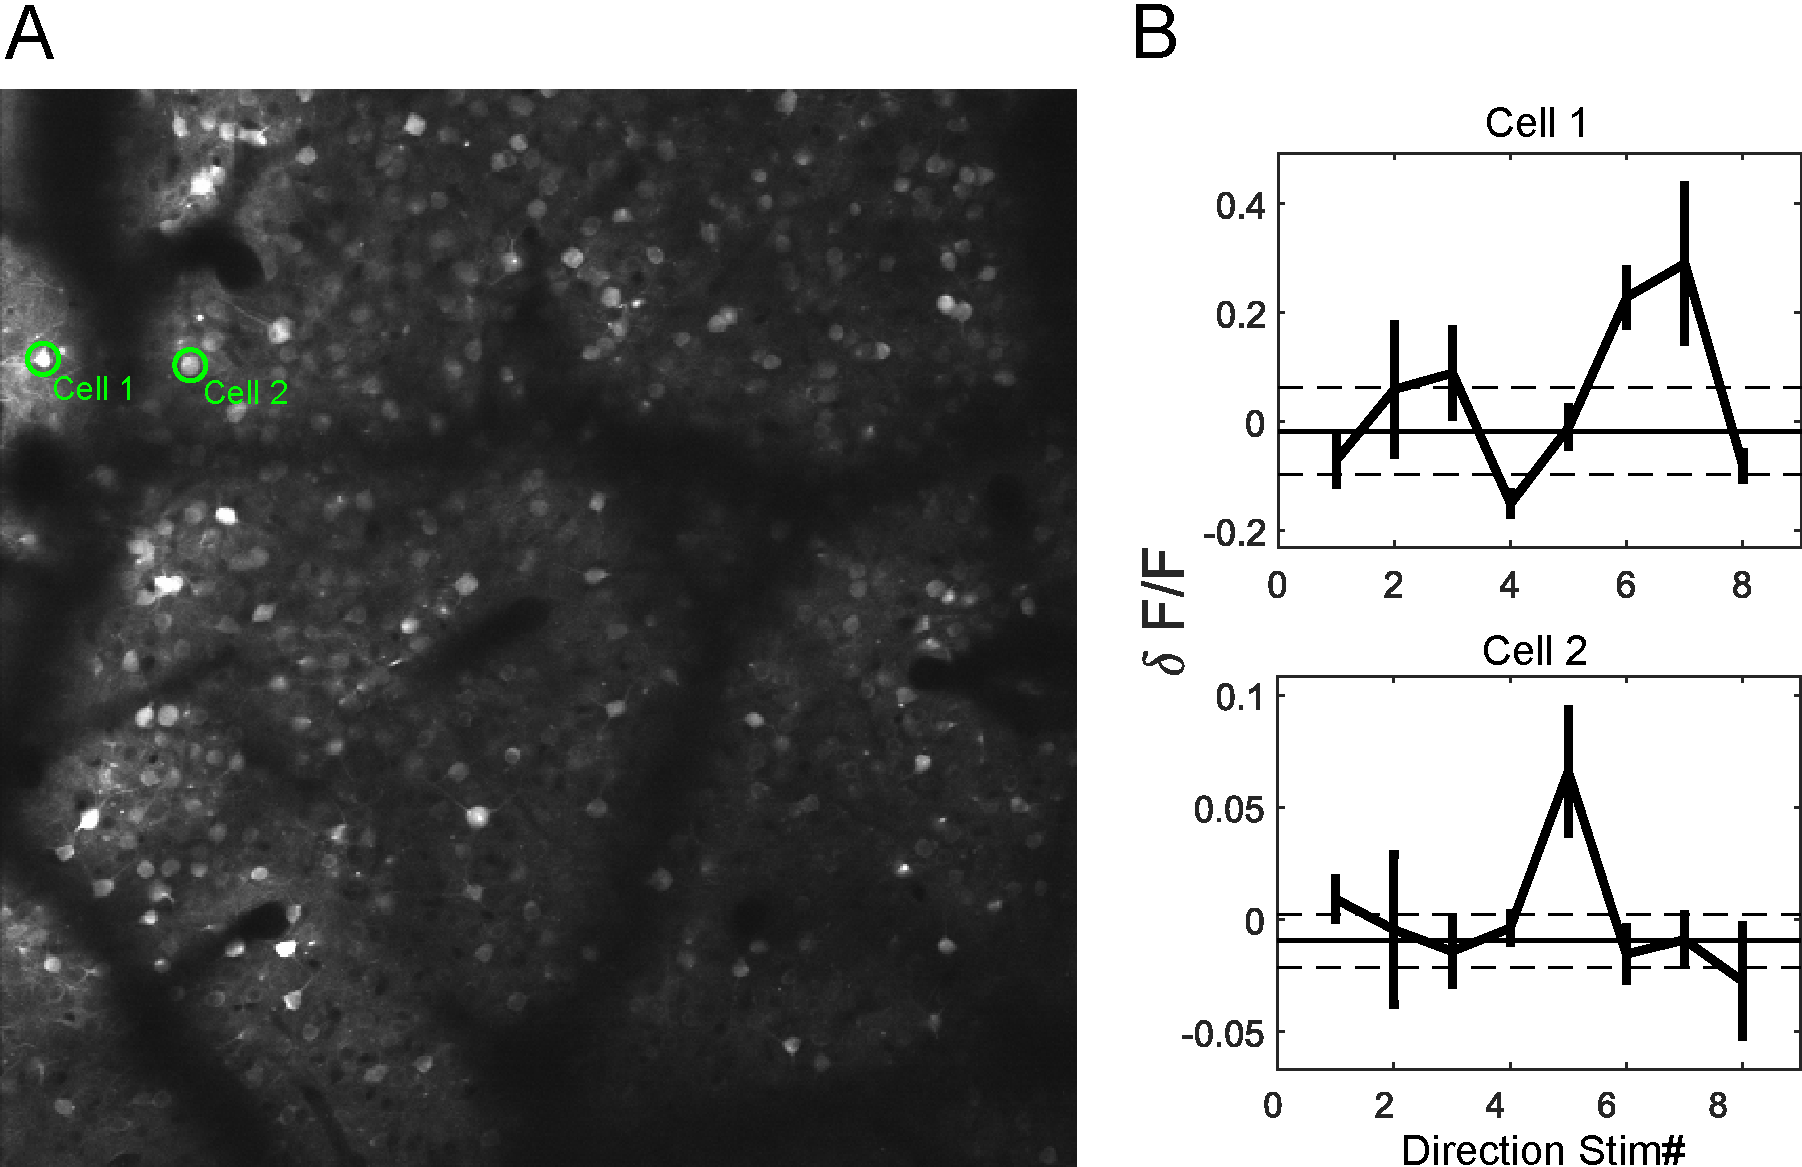
\includegraphics[width=\linewidth]{figures/_twophoton_responses.pdf}
  \caption{Two-photon calcium imaging of neuronal responses in
    ferret visual cortex.
    (\textit{A})~Representative time-averaged fluorescence image
    of a two-photon FOV in ferret V1. Cell bodies were manually
    identified using the \texttt{twophotonbulkload} GUI and are
    outlined as ROIs.
    (\textit{B})~Example direction tuning curves for
    two representative cells at selected SF~$\times$~TF
    conditions, illustrating the diversity of tuning profiles
    observed in the population. Error bars indicate
    $\pm$~SEM across trials.}
  \label{fig:example_cells}
\end{figure}


% ----------------------------------------------------------------
\section{Data Analysis}
\label{sec:analysis}
% ----------------------------------------------------------------

All analyses were performed in MATLAB R2024b
(MathWorks, Natick, MA) using custom scripts. Analysis code is available at \url{https://github.com/VH-Lab/vhlab-tpdirection-matlab} upon request.

% ---- 2.6.1  Visual responsiveness ----
\subsection{Visual Responsiveness}
\label{sec:responsiveness}

To identify visually responsive neurons, a one-way analysis of
variance (ANOVA) was performed for each cell, testing whether
the mean $\Delta F/F_0$ differed significantly across stimulus
conditions (including the blank condition). Cells were
classified as visually responsive if $p \leq 0.05$. Only
responsive cells were included in subsequent analyses. Across
all animals and FOVs, a total of [N] neurons were imaged, of
which [N] ([X]\%) met the responsiveness criterion and were
retained for analysis.

% ---- 2.6.2  Tuning curves ----
\subsection{Direction and Orientation Tuning Curves}

For each neuron and each SF~$\times$~TF combination, a
direction tuning curve was constructed by computing the mean
$\Delta F/F_0$ response across trials for each of the 8
directions. The orientation tuning curve was derived by
collapsing opposite directions (i.e., averaging responses at
$\theta$ and $\theta + 180^\circ$), yielding 4 orientation
conditions.

% ---- 2.6.3  Selectivity indices ----
\subsection{Direction and Orientation Selectivity Indices}

The direction selectivity index (DSI) was computed as the
normalized length of the mean resultant vector in direction
space:
%
\begin{equation}
  \text{DSI} \;=\;
    \frac{\left|\sum_{k} R_k \, e^{i\theta_k}\right|}
         {\sum_{k} R_k},
  \label{eq:dsi}
\end{equation}
%
where $R_k$ is the mean response to direction $\theta_k$ (in
radians), $i$ is the imaginary unit, and the sum runs over all
8 directions. DSI ranges from 0 (equal response to all
directions) to 1 (response to only one direction).

The orientation selectivity index (OSI) was computed
analogously, but with the direction angles doubled to map
orientation into a full circle:
%
\begin{equation}
  \text{OSI} \;=\;
    \frac{\left|\sum_{k} R_k \, e^{i \cdot 2\theta_k}\right|}
         {\sum_{k} R_k}.
  \label{eq:osi}
\end{equation}
%
DSI and OSI were computed separately at each SF~$\times$~TF
condition for every responsive cell.

% ---- 2.6.4  Preferred direction / orientation ----
\subsection{Preferred Direction and Orientation}

The preferred direction of each neuron at a given
SF~$\times$~TF condition was defined as the angle of the mean
resultant vector:
%
\begin{equation}
  \theta_{\text{pref}} \;=\;
    \arg\!\left(\sum_{k} R_k \, e^{i\theta_k}\right).
  \label{eq:prefdir}
\end{equation}
%
Similarly, the preferred orientation was computed as
%
\begin{equation}
  \phi_{\text{pref}} \;=\;
    \tfrac{1}{2}\,\arg\!\left(\sum_{k} R_k \,
      e^{i \cdot 2\theta_k}\right),
  \label{eq:prefori}
\end{equation}
%
which yields a value in the range $[0^\circ, 180^\circ)$.

% ---- 2.6.5  Delta-preference ----
\subsection{Shift in Preferred Direction and Orientation
  across Temporal Frequency}
\label{sec:delta_pref}

To quantify how feature preference changed with temporal
frequency, we computed the absolute shift in preferred
direction between two reference TF conditions. Unless
otherwise stated, the low-TF reference was 1.6~Hz and the
high-TF reference was 6.4~Hz, chosen because these conditions
were present across all recording sessions.

The absolute direction preference shift was defined as
%
\begin{equation}
  |\Delta\text{direction}| \;=\;
    \min\!\bigl(|\theta_{\text{pref}}^{\text{high}}
      - \theta_{\text{pref}}^{\text{low}}|,\;
    360^\circ - |\theta_{\text{pref}}^{\text{high}}
      - \theta_{\text{pref}}^{\text{low}}|\bigr),
  \label{eq:delta_dir}
\end{equation}
%
yielding a value in $[0^\circ, 180^\circ]$. An analogous
quantity, $|\Delta\text{orientation}|$, was computed using
preferred orientations and wrapped to $[0^\circ, 90^\circ]$.

These metrics were computed for all responsive cells at each
of the 5 spatial frequencies independently, to assess whether
the magnitude or prevalence of preference shifts depended on
SF.

% ---- 2.6.6  Functional maps ----
\subsection{Functional Preference Maps}

To visualize the spatial organization of feature preferences,
each neuron was plotted at its $(x_i, y_i)$ coordinates in the
FOV and color-coded by its preferred direction (using a
circular colormap spanning $0^\circ$--$360^\circ$) or preferred
orientation ($0^\circ$--$180^\circ$). Separate maps were
generated for each TF condition to allow visual comparison of
map topology across temporal frequencies.

Preference-shift maps were constructed by plotting
$|\Delta\text{direction}|$ as a vector at each cell's
location, with vector length proportional to the magnitude of
the shift and vector angle indicating the direction of the
shift. These maps were used to qualitatively assess whether
large preference shifts were spatially clustered or uniformly
distributed across the FOV.

% ---- 2.6.7  Pairwise spatial analysis ----
\subsection{Pairwise Spatial Analysis of Preference Shifts}
\label{sec:pairwise}

To quantify the spatial structure of preference shifts, we
computed pairwise statistics across all cell pairs within each
FOV. For each pair of neurons $i$ and $j$, we calculated the
Euclidean distance $d_{ij}$ between their spatial coordinates
(in pixels) and the absolute difference in their direction
preference shifts,
$|\Delta\text{dir}_i - \Delta\text{dir}_j|$.

These pairwise measurements were binned by inter-cell distance
into 20 equally spaced bins spanning 0 to 500 pixels, and the
mean $|\Delta\text{shift}|$ was computed within each distance
bin. This analysis tests whether nearby cells undergo more
similar preference shifts than distant cells, which would
indicate a spatially organized mechanism underlying
TF-dependent retuning.

[If you used a statistical test: Significance of the
distance--similarity relationship was assessed using a
permutation test (N = 1000 shuffles). The null distribution
was generated by randomly permuting cell identities while
preserving the spatial layout, thereby destroying any spatial
structure in $\Delta\text{shift}$ while maintaining the overall
distribution of pairwise distances.]


% ================================================================
%  BIBLIOGRAPHY ENTRIES NEEDED (add to your .bib file):
%
%  VanHooser2015 — Van Hooser SD, Johnson EN, Li Y, et al.
%    "Practical Methods for In Vivo Cortical Physiology with
%    2-Photon Microscopy and Bulk Loading of Fluorescent
%    Calcium Indicator Dyes." Neuroscience Methods, 2015.
%
%  Smith2016 — Smith GB, Whitney DE, Fitzpatrick D.
%    "Viral Injection and Cranial Window Implantation for
%    In Vivo Two-Photon Imaging." Neuroscience Methods, 2016.
%
%  GarciaMurillo2022 — García Murillo D, Rogovin O, et al.
%    "NDI: A platform-independent data interface and database
%    for neuroscience physiology and imaging experiments."
%    eNeuro, 2022.
%
%  Brainard1997 — Brainard DH. "The Psychophysics Toolbox."
%    Spatial Vision, 1997.
%
%  Pelli1997 — Pelli DG. "The VideoToolbox software for visual
%    psychophysics." Spatial Vision, 1997.
% ================================================================

% ================================================================
%  Figure placements for Methods
% ================================================================


\chapter{Results}

\begin{figure}[t]
    \centering
    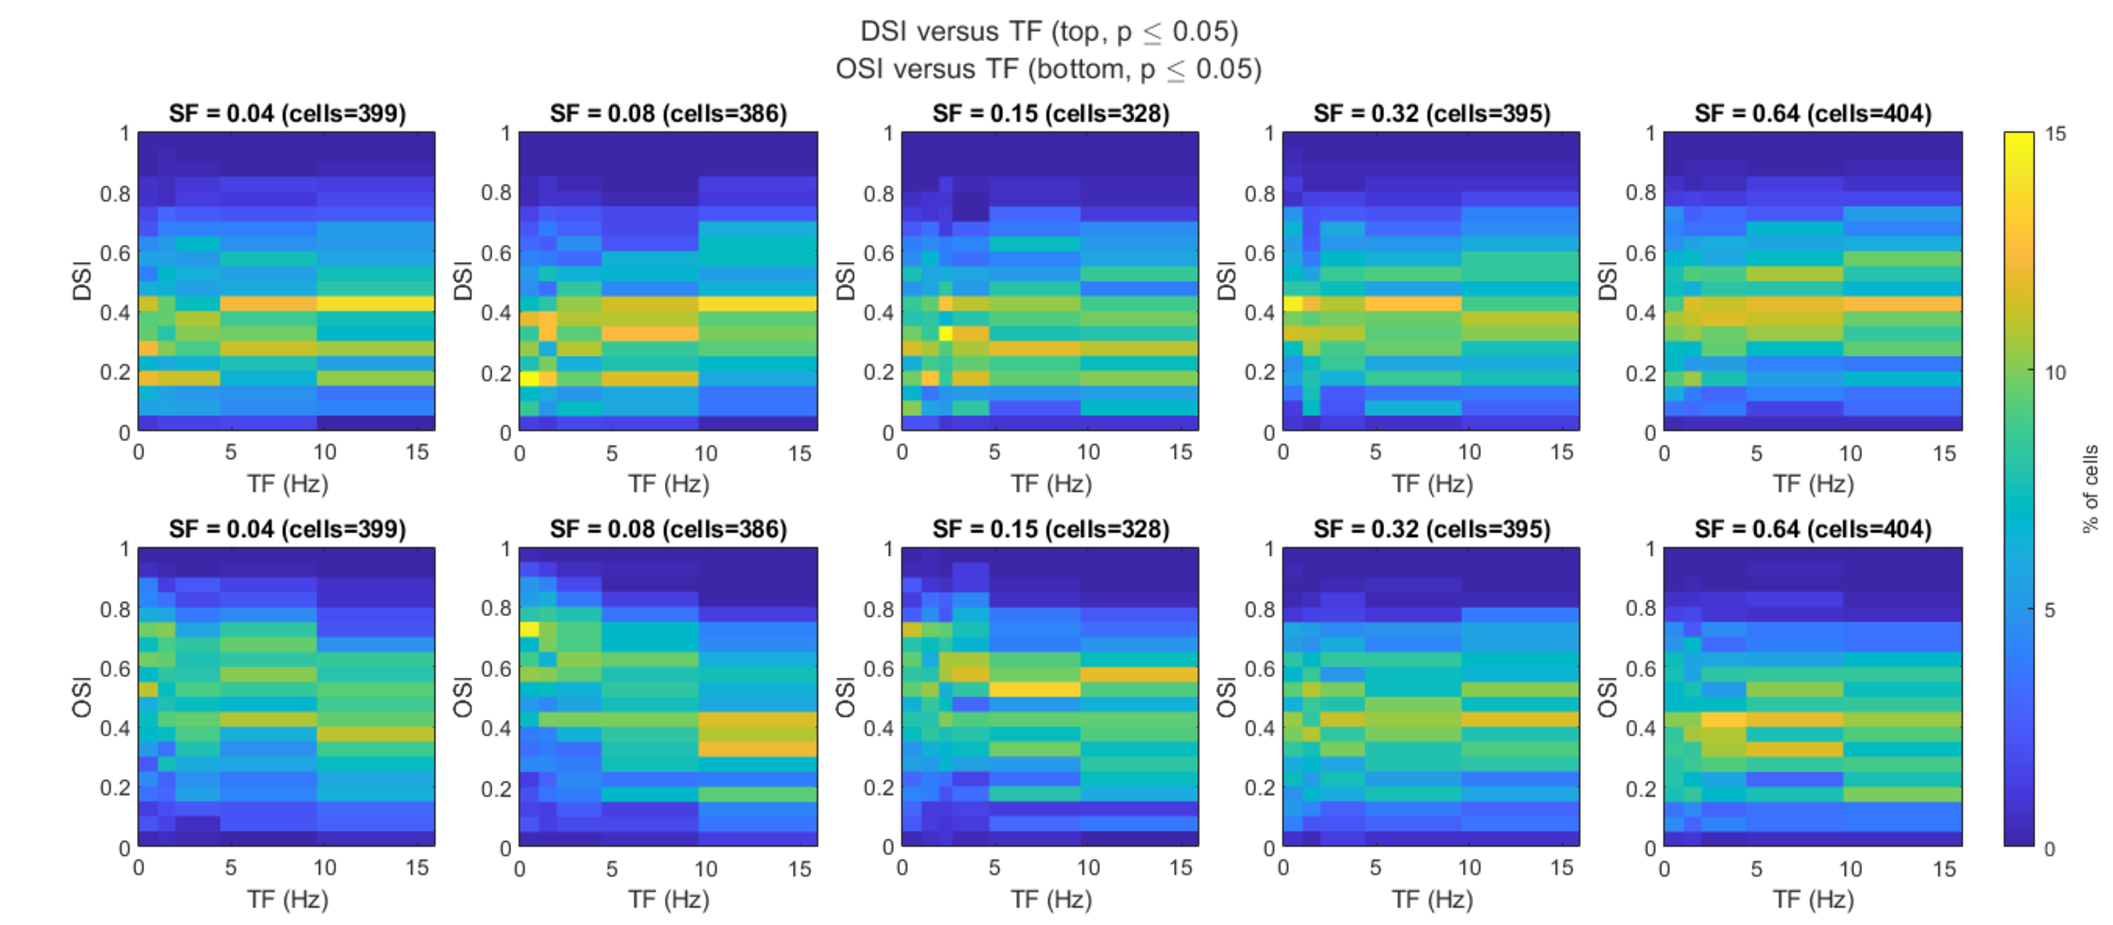
\includegraphics[width=1\linewidth]{figures/_DSI_OSI_vs_TF.pdf}
    \caption{Population distributions of direction and orientation 
    selectivity as a function of temporal frequency, across five spatial frequencies. Each panel shows a 2D histogram (color indicates cell count) of selectivity index versus TF (Hz) for cells with $p \leq 0.05$. \textit{Top row}: Direction selectivity index (DSI) versus TF for SF = 0.04, 0.08, 0.15, 0.32, and 0.64 cyc/deg (left to right; $n = 399, 386, 328, 395, 404$ cells, respectively). \textit{Bottom row}: Orientation selectivity index (OSI) versus TF for the same spatial frequencies and cell counts.}
    \label{fig:dsi_osi_heatmaps}
\end{figure}




\chapter{Discussion}

Discussion body paragraphs



% Put references in a singlespacing environment so it goes back to double for the appendices
\begin{singlespacing}
\bibliographystyle{plainnat}
\bibliography{main}
\end{singlespacing}


% If you don't have appendices, remove this command and the chapter below
\appendix

\chapter{Supplementary Material}

\section{Details}

Lorem ipsum dolor sit amet, consectetur adipiscing elit. Sed dapibus metus in erat varius tincidunt. Nulla diam neque, fringilla a interdum id, vehicula id erat. Vestibulum ante ipsum primis in faucibus orci luctus et ultrices posuere cubilia curae; Mauris elementum odio orci. Nam at velit id augue tempus hendrerit. Fusce vestibulum purus eget eros semper, et consectetur libero pellentesque. Phasellus ultricies malesuada erat fringilla luctus. Sed vel sapien vitae diam vestibulum imperdiet non eget nisi.

Fusce suscipit eros ligula. Mauris faucibus in massa nec malesuada. Mauris sit amet vestibulum nibh. Phasellus libero nisl, viverra id tempor vel, ornare id tortor. Nunc at sem a leo tempus dictum. In sed dignissim ipsum. Aenean condimentum vestibulum ligula, et viverra urna. Mauris in risus et nulla lobortis pretium ac a neque. Etiam porttitor enim nec ornare placerat. Proin faucibus nibh eu magna convallis pellentesque.


\begin{figure}[t]
    \centering
    This is where a figure would go.
    \caption{Sample appendix figure.}
    \label{fig:sampleappendix}
\end{figure}

Curabitur nec porttitor tortor, eget hendrerit nisl. Vestibulum et lobortis lacus. Donec porta iaculis dolor, in sollicitudin mauris. Pellentesque eget consectetur tellus. Sed a hendrerit turpis. Morbi rhoncus pulvinar mauris, at rutrum eros egestas vel. Aliquam sapien sapien, efficitur nec pharetra eget, vehicula sit amet sapien. Integer in risus nec massa feugiat volutpat vitae vel libero. Phasellus ornare, mauris a maximus pretium, quam nisl mattis nulla, sit amet convallis lectus est a urna.

Quisque enim velit, mollis aliquet posuere at, convallis id tellus. Ut consectetur cursus ligula eget hendrerit. Proin vitae porta sapien, ac dapibus justo. Nulla tincidunt quis eros ut tincidunt. Curabitur aliquam nulla tortor, eu vehicula sem volutpat ut. Suspendisse potenti. Quisque sit amet sapien molestie, blandit est ut, viverra sem. Maecenas dignissim maximus vestibulum. Integer varius risus in justo tincidunt malesuada. Etiam tempor eleifend arcu eget pellentesque.

\end{document}
